%\documentclass{article}
\documentclass[a4paper]{article}
\fontencoding{T1}
\usepackage{anysize}
\usepackage{cite}
%\marginsize{left}{right}{top}{bottom}
\marginsize{1.8cm}{1.8cm}{1.5cm}{1.5cm}
%\usepackage[spanish,activeacute]{babel}
\usepackage{cite}
\usepackage{pdflscape}
\usepackage{epsfig}
\usepackage{amsfonts}
\usepackage{amsmath}
\usepackage{amssymb}
\usepackage{color}
\usepackage{graphicx} % Allows including images


\begin{document}


\title{Manuelita vivia en Pehuajo}
\author{all}

%\date{\small{$^{\S}$ Instituto de Física de Líquidos y Sistemas Biológicos
%Instituto de Investigaciones Fisicoqu\'{i}micas Te\'{o}ricas y Aplicadas (INIFTA), Universidad Nacional de La Plata, CCT La Plata - CONICET, Argentina.}}
\maketitle

\begin{abstract}

sasa

\end{abstract}



\section*{Introduction}



\section*{Methodology}



\section*{Results and Discussion}
The distance traveled as a function of time was calculated from the $(\mathrm{latitude}, \mathrm{longitude})$ data by determining the distance on the Earth's surface using the Haversine function.

The total accumulated distance traveled was then calculated as:

\[
\mathrm{distot}(t)=\mathrm{distot}(t-1)+\mathrm{distance}(t)
\]

Figure \ref{fig1} shows all the measured quantities for turtle T10. There are some temporal gaps corresponding to missing data.

A similar behavior is observed for the other turtles (T6, T12, T30, T54, T79, T128, T185, and T206).


\begin{figure}[!h]
\begin{center}
\includegraphics[width=10cm,clip=true,angle=0]{tortuga10.eps}
\end{center}
\caption{Datos de la Tortuga T10: A) Datos crudos de (lat,long) ; B) Lo mismo que en A) pero metros, para chequear que el pasaje de datos funcione. C) Distancia recorrida (cada 15min) en funcion del tiempo; D) Distancia acumulada vs time: los colores indican los exponentes del ajuste en cada periodo. }
\label{fig1}
\end{figure}

The distances traveled by the turtles were measured every 15 minutes.
Based on the observed behavior, we can define an exponent as:

\begin{equation}
{\rm P(d)} \approx d^{-\beta}
\label{eq:pd}
\end{equation}

The mean exponent for the 9 turtles is: $\beta = 2.1(2)$, as shown in Figure \ref{fig22}.

\begin{figure}[!h]
\begin{center}
\includegraphics[width=10cm,clip=true,angle=0]{HistoNorm.eps}
\end{center}
\caption{ Distribucion de distancias recorridas cada $\Delta t=15min$.}
\label{fig22}
\end{figure}

La nueva figura, comparando los datos completos y solo hora solar (9 a 17hs) Figure \ref{fig222}.
\begin{figure}[!h]
\begin{center}
\includegraphics[width=10cm,clip=true,angle=0]{Histogram_new.eps}
\end{center}
\caption{ Distribucion de distancias recorridas cada $\Delta t=15min$.}
\label{fig222}
\end{figure}


\subsection*{Mean square deviation (MSD)}

By calculating the MSD for each tortoise, markedly different behaviors are observed, both among tortoises and depending on the time period (Figure \ref{fig3}).
We can fit an exponent:
\begin{equation}
{\rm {MSD}} \approx t^{\alpha }
\label{eq:msd}
\end{equation}


\begin{figure}[!h]
\begin{center}
\includegraphics[width=10cm,clip=true,angle=0]{msd_dist.eps}
\end{center}
\caption{All turtles (identified as Tnumber): MSD versus time. The dotted black line has a slope corresponding to $\alpha \approx t^{0.8}$.} 
\label{fig3}
\end{figure}

The data suggest that, at least during certain periods, the behavior is subdiffusive ($\alpha < 1$).

\subsection*{Seasonality}

If we attempt to separate the behavior according to biological/climatic periods, namely: November--January, February--March, and April--October, we observe that the MSD behavior is markedly different, with exponents ranging from subdiffusive to diffusive regimes. Figure \ref{fig24} shows only the case for T10.
The seasonal periods still need to be refined. Here, only the calendar months were considered, but factors such as temperature, late spring conditions, and related environmental variables should probably also be taken into account.


\begin{figure}[!h]
\begin{center}
\includegraphics[width=10cm,clip=true,angle=0]{T10estaciones.eps}
\end{center}
\caption{Separacion estacional de T10.}
\label{fig24}
\end{figure}

Para todas las tortugas el MSD Figure \ref{fig25} y la distribucion de distancias $P(d)$ Figure \ref{fig26}


\begin{figure}[!h]
\begin{center}
\includegraphics[width=10cm,clip=true,angle=0]{msdtodasT.eps}
\end{center}
\caption{MSD segun separacion estacional para todas las tortugas.}
\label{fig25}
\end{figure}


\begin{figure}[!h]
\begin{center}
\includegraphics[width=10cm,clip=true,angle=0]{distribDistodasT.eps}
\end{center}
\caption{Distribucion de distancias recorridas en intervalos de 15min segun separacion estacional para todas las tortugas}
\label{fig26}
\end{figure}

In both figures, Fig.~\ref{fig25} and Fig.~\ref{fig26}, the dotted lines correspond to the best fits obtained. Table~1 lists the values of these exponents ($MSD(t) \approx t^{\alpha}$ and $P(d) \approx d^{-\beta}$). As can be seen, there is considerable dispersion among turtles and across different periods of the year.

It should be noted that for some tortoises (T128, T185, and T206) only limited data are available. For example, no data are available for the November--January period, and for the April--October period only data from the first months (April and May) are available, as indicated in Figures \ref{fig25} and \ref{fig26}.

\begin{figure}[!h]
\begin{center}
\includegraphics[width=12cm,clip=true,angle=0]{alfa_beta.eps}
%\includegraphics[width=7cm,clip=true,angle=0]{beta.jpg}
\end{center}
\caption{Table 1: Exponents of MSD and $P(d)$ for each turtle and for each period. Males and females are distinguished by color, and the exponents were calculated using all available data.}
\label{tabla1}
\end{figure}


\subsection*{Males and females}

So far, the MSD appears to exhibit a power-law behavior during the February--March period. Beyond this interval, it becomes difficult to obtain reliable fits.

Within this period, it may be useful to separate the data between males and females in order to investigate possible differences.

Figure \ref{figMH1} shows the MSD behavior separated by males and females. The exponent $\alpha$ (Eq.~\ref{eq:msd}) does not appear to change significantly between males and females; rather, there is considerable dispersion in the data (see Table~2).

A similar situation is observed for the distribution of traveled distances (Figure \ref{figMH2}), although in this case the dispersion in the curves may be larger among females than among males.

Table~2 lists the values of the exponents.

\begin{figure}[!h]
\begin{center}
\includegraphics[width=10cm,clip=true,angle=0]{MSD-MH.eps}
\end{center}
\caption{MSD separated in males and females}
\label{figMH1}
\end{figure}



\begin{figure}[!h]
\begin{center}
\includegraphics[width=10cm,clip=true,angle=0]{HistoNormM-H.eps}
\end{center}
\caption{P(d) vs d separated in males and females}
\label{figMH2}
\end{figure}



\begin{figure}[!h]
\begin{center}
\includegraphics[width=6cm,clip=true,angle=0]{tabla_exponentes.eps}
\end{center}
\caption{Table 2: MSD and $P(d)$ exponents for each tortoise, separated by males and females, calculated using all available data without separation by periods.}
\label{tabla2}
\end{figure}


\section*{Bouts of walking behaviour}

We have shown that the power-law distribution of displacements can be explained by assuming the tortoise performs random walks with constant speed interspersed with resting periods, provided the duration of the walking bouts is distributed with a power-law, or Pareto, distribution,
$$  P_b(t) = \frac{\alpha-1}{t^\alpha}, \qquad t\ge1, $$
where \(P_b(t)\,dt\) is the probability that a bout of walking will last from time \(t=0\) to a time between \(t\) and \(t+dt\).

This behaviour can also be explained by considering the transition probability from walking to resting, \(\gamma(t)\).  The transition probability is the probability that the tortoise will stop walking at a time between \(t\) and \(t+dt\), given that it is walking at time \(t\), i.e.
$$ \gamma(t) = \frac{P_b(t)}{\text{P. of walking at time $t$}} = \frac{P_b(t)}{1 - \text{P. of having stopped between $0$ and $t$}} = \frac{P_b(t)}{1-\int_0^t\!\!P_b(t')\,dt´} . $$
Since \(\int_1^t (\alpha-1) t^{-\alpha} = 1 - t^{1-\alpha}\), we obtain
$$ \gamma(t) = \frac{\alpha-1}{t},  t\ge1, $$
i.e.$\backslash$ the probability that the tortoise will decide to rest gets smaller the longer it has been walking.

Power-law-distributed bouts of behaviour have been discussed before  \cite{falligant2024}, \cite{gomez2026}, but not everyone seems to agree on power laws \cite{breed2015}.



\section*{Supplement}
By testing a different temporal interval, $\Delta t = 30\,\mathrm{min}$, the exponent does not change, nor is any improvement observed in $P(d)$ (Figure \ref{fig23}).

\begin{figure}[!h]
\begin{center}
\includegraphics[width=10cm,clip=true,angle=0]{histo15_30.eps}
\end{center}
\caption{Distribution of traveled distances for T185, using $\Delta t = 15\,\mathrm{min}$ and $\Delta t = 30\,\mathrm{min}$.}
\label{fig23}
\end{figure}

\end{document}

